\subsection{write}
\subsubsection{write函数整体介绍}
write函数通常用于将数据从用户空间写入文件或其他的输出设备,如果文件不可写,则返回相应的错误类型。
\noindent
write的参数与返回值展示如下:
\begin{lstlisting}[language={Rust}, 
    caption={write的参数与返回值}]
pub fn sys_openat(dirfd: usize, path: *const u8, flags: u32, mode: u32) -> isize
\end{lstlisting}
解释如下:
\begin{itemize}
    \item fd 表示文件描述符,一般通过open函数的返回值获得,对当前任务队列的活跃文件进行唯一标识。
    \item buf 表示写入数据的缓冲区的指针。
    \item count 表示要写入的字节数,和buf参数一起可以表示写入数据的全部内容。
\end{itemize}
\subsubsection{整体流程}
流程图展示如下:
\begin{figure}[H]
    \centering
    \scalebox{0.5}{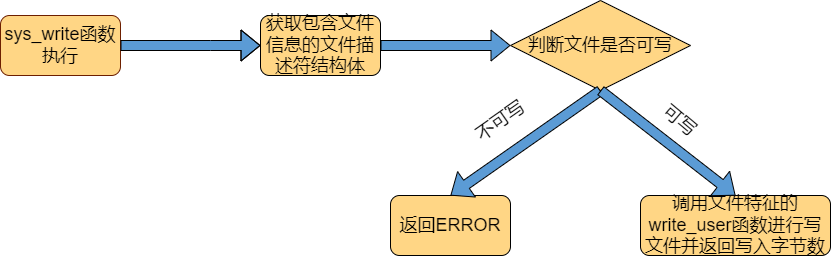
\includegraphics{figures/09-04-write-流程图.png}}
    \caption{wtire流程图}
\end{figure}

\subsubsection{代码详析}
1、函数输入参数展示如下:
\begin{lstlisting}[language={Rust},
    caption={write的参数与返回值}]
    pub fn sys_write(fd: usize, buf: usize, count: usize) -> isize
\end{lstlisting}

2、获取TCB信息并通过get_ref函数和得到的文件描述符表fd_table,将参数fd转化成包含文件信息的文件描述符结构体指针file_descriptor。
\begin{lstlisting}[language={Rust},
    caption={含有文件信息文件描述符指针的获取}]
    let task = current_task().unwrap();
    let fd_table = task.files.lock();
    let file_descriptor = match fd_table.get_ref(fd) {
        Ok(file_descriptor) => file_descriptor,
        Err(errno) => return errno,
    };
\end{lstlisting}

3、判断文件是否可写,如果不可写则返回EBADF。(Bad file number,值为-9)
\begin{lstlisting}[language={Rust},
    caption={文件权限判断}]
    if !file_descriptor.writable() {
        return EBADF;
    }
\end{lstlisting}

4、获取用户空间令牌,用于下文缓冲区数据的获取。

\begin{lstlisting}[
    language={Rust},
    caption={获取用户空间令牌}
]
let token = task.get_user_token();
    
\end{lstlisting}

5、通过调用write_user函数,将用户空间数据写入文件描述符对应的文件中。
write_user有两个参数:
\begin{lstlisting}[
    language={Rust},
    caption={write_user参数}
]
fn write_user(&self, offset: Option<usize>, buf: UserBuffer) -> usize
\end{lstlisting}
\begin{itemize}
    \item offset 表示用户指定的固定偏移量(相对于文件开始位置的偏移),不受文件指针偏移的影响。
    \item buf 表示一个UserBuffer结构体,其内部信息通过translated_byte_buffer函数获得。
\end{itemize}
    UserBuffer结构体内容如下,包括一个表示数据具体内容的Vec<\&mut[u8]> 和表示长度的len。
\begin{lstlisting}[
    language={Rust},
    caption={UserBuffer结构体}
]
pub struct UserBuffer {
    /// The segmented array, or, a "vector of vectors".
    /// # Design Information
    /// In Rust, reference lifetime is a must for this template.
    /// The lifetime of buffers is `static` because the buffer 'USES A' instead of 'HAS A'
    pub buffers: Vec<&'static mut [u8]>,
    /// The total size of the Userbuffer.
    pub len: usize,
}
    
\end{lstlisting}

translated_byte_buffer函数接受三个参数,用户空间令牌token,缓冲区指针ptr和缓冲区长度len,返回值为一个Result包裹的Vec<\&mut[u8]>变量。

\begin{lstlisting}[
    language={Rust},
    caption={translated_byte_buffer函数的参数和返回值}
]
pub fn translated_byte_buffer(
    token: usize,
    ptr: *const u8,
    len: usize,
) -> Result<Vec<&'static mut [u8]>, isize> 
    
\end{lstlisting}

6、深入文件描述符的write_user函数,我们以OSInode的实现为例进行讲解。
首先初始化写入总字节数变量total_write_size并获取文件的写锁。接下来分两种情况进行处理,
如果偏移量不为None,则通过循环遍历用户缓冲区,调用self.inner.write_at_block_cache_lock函数
分次将数据写入文件,同时确保实际写入的字节数与数据片段长度相等,并维护偏移量offset(指向下一个位置)和写入总字节数total_write_size。
\begin{lstlisting}[
    language={Rust},
    caption={偏移量不为None}
]
Some(mut offset) => {
    let mut offset = &mut offset;
    for slice in buf.buffers.iter() {
        let write_size =
            self.inner
                .write_at_block_cache_lock(&inode_lock, *offset, *slice);
        assert_eq!(write_size, slice.len());
        *offset += write_size;
        total_write_size += write_size;
    }
}
\end{lstlisting}

如果偏移量为None,则需额外对offset进行处理,如果不是追加模式则设置offset为文件描述符的偏移量,如果为追加模式则将offset设置为文件的当前大小,其余的操作与offset不为None的情况相同。
\begin{lstlisting}[
    language={Rust},
    caption={偏移量为None的情况}
]
None => {
    let mut offset = self.offset.lock();
    if self.append {
        *offset = self.inner.get_file_size_wlock(&inode_lock) as usize;
    }
    for slice in buf.buffers.iter() {
        let write_size =
            self.inner
                .write_at_block_cache_lock(&inode_lock, *offset, *slice);
        assert_eq!(write_size, slice.len());
        *offset += write_size;
        total_write_size += write_size;
    }
}
\end{lstlisting}
7、我们继续深入,来分析write的块级实现write_at_block_cache_lock,它接受三个参数:

\begin{itemize}
    \item inode_lock 表示文件的写锁。
    \item offset 表示写数据位置的偏移量,即写数据位置相对文件开始位置的偏移。
    \item buf 表示具体要写入文件的数据,类型为\&[u8]。
\end{itemize}

write_at_block_cache_lock函数首先通过获得的偏移量的信息来判断是否需要进行空间的扩展,如果diff_len大于0,则调用modify_size_lock扩展diff_len大小的空间。(分配新簇)
\begin{lstlisting}[
    language={Rust},
    caption={判断是否进行空间扩展分配}
]
let mut start = offset;
        let old_size = self.get_file_size() as usize;
        let diff_len = buf.len() as isize + offset as isize - old_size as isize;
        if diff_len > 0 as isize {
            // allocate as many clusters as possible.
            self.modify_size_lock(inode_lock, diff_len, false);
        }
\end{lstlisting}

接着计算写入结束位置end并确保start小于end,同时初始化写入的缓存块索引 start_cache 和写入的总字节数 write_size。

\begin{lstlisting}[
    language={Rust},
    caption={其他变量初始化}
]
let end = (offset + buf.len()).min(self.get_file_size() as usize);

debug_assert!(start <= end);

let mut start_cache = start / PageCacheManager::CACHE_SZ;
let mut write_size = 0;
\end{lstlisting}

最后循环处理并写入数据块缓存,每次循环维护当前数据块的结束位置end_current_block,并通过get_cache方法获取数据块的缓存,调用modify将数据从用户提供的缓冲区buf复制到数据块缓存,
同时维护写入字节数和数据块的写入位置。

\begin{lstlisting}[
    language={Rust},
    caption={循环处理数据块并写入}
]
loop {
    // calculate end of current block
    let mut end_current_block =
        (start / PageCacheManager::CACHE_SZ + 1) * PageCacheManager::CACHE_SZ;
    end_current_block = end_current_block.min(end);
    // write and update write size
    let lock = self.file_content.read();
    let block_write_size = end_current_block - start;
    self.file_cache_mgr
        .get_cache(
            start_cache,
            || -> Vec<usize> { self.get_neighboring_sec(&lock.clus_list, start_cache) },
            &self.fs.block_device,
        )
        .lock()
        // I know hardcoding 4096 in is bad, but I can't get around Rust's syntax checking...
        .modify(0, |data_block: &mut [u8; 4096]| {
            let src = &buf[write_size..write_size + block_write_size];
            let dst = &mut data_block[start % PageCacheManager::CACHE_SZ
                ..start % PageCacheManager::CACHE_SZ + block_write_size];
            dst.copy_from_slice(src);
        });
    drop(lock);
    write_size += block_write_size;
    // move to next block
    if end_current_block == end {
        break;
    }
    start_cache += 1;
    start = end_current_block;
}
\end{lstlisting}